% This file is part of the openLilyLib project
% Copyright Urs Liska 2013
% This file and the resulting PDF document aren't distributed under a free license.
% You may freely redistribute both the source and the pdf 
% without modifications, however.

\documentclass[DIV=12]{scrreprt}

\usepackage{scrpage2}
\pagestyle{scrheadings}
\rohead{\textcolor{red}{\textsc{Entwurf} -- bitte nicht weitergeben!}}
\cohead{}

\usepackage{fontspec}

% Language settings
\usepackage{polyglossia}
\setdefaultlanguage{german}
\frenchspacing

% fontspec base settings
\defaultfontfeatures{%
	Ligatures=TeX
}
\setmainfont[%
	Numbers=OldStyle,
	]{Minion Pro}
\setsansfont[Scale=MatchLowercase,]{Cronos Pro}
\setmonofont[Scale=MatchLowercase]{Inconsolata}

% Typographical improvements
\RequirePackage{microtype}
\RequirePackage[ngerman]{selnolig}

\linespread{1.05}

\RequirePackage{lilyglyphs}

\RequirePackage{xmpFancyref}
\RequirePackage{musicexamples}

\RequirePackage{hologo}

% Do not restart footnote numbering for each chapter
\RequirePackage{chngcntr}
\counterwithout*{footnote}{chapter}

% Enhanced lists
\RequirePackage{mdwlist}
\RequirePackage{paralist}

% Multicolumn texts
\RequirePackage{multicol}

% Extended verbatim (listing) texts
\RequirePackage{fancyvrb}
\usepackage{listings}
\usepackage{OLLstyles}

%%%%%%%%%%%%%%%%%%%%%%%%%%%
% Options for use of hyperlinks
% (make sure this is included last)
\RequirePackage[%
	colorlinks,
	urlcolor=blue,
	bookmarks=true,
	bookmarksnumbered=true]{hyperref}



\begin{document}
\title{Reintext-basiertes Arbeiten\\für Musikwissenschaftler}
\author{Urs Liska}
\maketitle

\subsection*{Vorbemerkung}
Eine große Mehrheit an Partituren und musikwissenschaftlichen Textdokumenten entsteht mit Hilfe grafischer Anwendungsprogramme, und den meisten Autoren dürfte die Existenz einer grundsätzlichen Alternative überhaupt nicht bewusst sein.
Der vorliegende Aufsatz zeigt demgegenüber einen Ansatz, der auf der Bearbeitung reiner Textdateien basiert.
Dieser Ansatz, der Erfahrungen und Strategien aus der Softwareentwicklung für unsere Disziplinen fruchtbar macht, ermöglicht neuartige Wege gemeinschaftlichen Arbeitens, Forschens und Publizierens.
Die beschriebenen Konzepte, Werkzeuge und Arbeitsprozesse haben mein Leben als Autor von Text- und Partiturdokumenten grundlegend verändert, und es ist mir ein großes Anliegen, sie der musikwissenschaftlichen Gemeinschaft vorstellen.

In den Geisteswissenschaften ist textbasiertes Arbeiten weitgehend unbekannt, während es in vielen natur- und computerwissenschaftlichen Disziplinen zum Standard gehört.
Tatsächlich erfordert das Arbeiten mit Reintextdateien ein grundlegendes Umdenken, was wohl auch die erheblichen Vorbehalte erklärt, mit denen die entsprechenden Techniken meist zur Kenntnis genommen werden.
Allerdings erscheint mir diese Zurückhaltung nur bedingt gerechtfertigt, denn die Konzepte, mit denen wir uns berufsbedingt auseinandersetzen -- seien es Fingersätze oder Quellenbeschreibungen -- sind nicht weniger komplex.
Insgesamt betrachte ich die Auseinandersetzung mit textbasierten Programmen und Ansätzen als eine überaus lohnende und gerechtfertigte Investition, insbesondere, wenn sie nicht als Einzelaspekt, sondern im Zusammenhang betrachtet werden.
Auf lange Sicht kann textbasiertes Arbeiten die musikwissenschaftliche Produktivität sowie die Qualität der Ergebnisse erhöhen.
Ein grundlegendes Interesse hier- sowie Verständnis dafür möchte ich mit diesem Aufsatz herstellen.

\medskip
Das vorliegende Dokument ist die stark verkürzte Fassung eines englischen Beitrags, der in dem Blog \emph{Scores of Beauty} veröffentlicht wurde%
\footnote{\url{http://lilypondblog.org/2013/07/plain-text-files-in-music/}}.
Die Idee des Originals ist eine möglichst behutsame Einführung in das Thema für jeden, der mit der Erstellung von Musik-Texten und Partituren befasst ist, während die Kurzversion deutlicher auf die musikwissenschaftliche Perspektive zugespitzt ist.
Insbesondere möchte ich die komplexeren Aspekte und Potenziale bei institutionellen Rahmen- und Arbeitsbedingungen herausarbeiten.
Bei Verständnisfragen empfehle ich daher, auf die nahezu gleich strukturierte englische 
Fassung zurückzugreifen.

Die wesentlichen Softwaresysteme, die ich auf den folgenden Seiten vorstellen -- in deren Benutzung ich aber nicht einführen -- werde, sind:

\begin{itemize*}
\item \emph{Versionsverwaltung} -- behält die Übersicht über Ihre Arbeit
\item \emph{LilyPond} -- das Notensatzprogramm
\item \emph{\LaTeX} -- das professionelle Textsatzsystem
\end{itemize*}

Außer dem Verfassen von Text- und Partiturdokumenten spielen im Zusammenhang mit musikwissenschaftlichem Arbeiten noch weitere Technologien (wie etwa Datenbanken und Webserver) eine Rolle, die an dieser Stelle jedoch nicht erörtert werden.

\vfill
\hrule
\medskip
\textcopyright{} Urs Liska 2013 -- Weitergabe des unveränderten Dokuments gestattet.

\tableofcontents

\chapter{Textformate}
\label{chap:pt_plain-text-format}
„Traditionelle“, grafische Programme bilden den gesamten Arbeitsprozess bei der Erstellung von Dokumenten in einer \textsc{wysiwig%
\footnote{What You See Is What You Get -- die Bildschirmdarstellung gleicht der endgültigen Ausgabe auf Papier}}-Umgebung ab.
Demgegenüber ist bei der Bearbeitung von Textdateien das Ergebnis nicht unmittelbar ersichtlich -- der „Quelltext“ muss erst in ein grafisches Dateiformat „übersetzt“ oder „kompiliert“ werden.
Weshalb sollte man sich nun diese Abstraktionsebene aufbürden, wo es doch offensichtlich schnell, einfach und effizient ist, ein Dokument in seinem endgültigen Erscheinungsbild zu bearbeiten?
Ist es nicht nachgerade \emph{natürlich}, eine Partitur grafisch zu bearbeiten?

Nun, es gibt eine Reihe guter Gründe, Dokumente als Textdateien zu speichern und zu bearbeiten.
Textbasiertes Arbeiten umgeht einige grundlegende Probleme anderer Ansätze, und es eröffnet Perspektiven auf ein breites Spektrum erweiterter Möglichkeiten.
Und schließlich gibt es heutzutage Bearbeitungsprogramme, welche den Umgang mit Textdateien erheblich vereinfachen.

Einleitend werde ich einige grundlegende Aspekte der Verwendung von Reintextformaten erläutern, doch vorab eine Bemerkung zur Terminologie.
Da es bei diesem Thema eine Reihe von Mehrdeutigkeiten gibt, werde ich im Folgenden einige selbstgewählte Regeln beachten:
Wenn ich von \emph{Dateien} spreche, meine ich die physische Speicherung auf einer Festplatte, während \emph{Dokument} die konzeptionelle Einheit bezeichnet.
Ein \emph{Textdokument} ist somit beispielsweise der vorliegende Aufsatz, unabhängig von dem Dateiformat, in dem er gespeichert ist.
\emph{Textdatei} (oder auch \emph{Reintextdatei}) bezeichnet dagegen eine physische Datei, in der ausschließlich Reintext gespeichert ist.
Auf das zweideutige „Text“ versuche ich nach Möglichkeit zu verzichten.

\section{Inhalt, Bedeutung und Erscheinungsbild}
\label{sec:pt_separation-content-meaning-appearance}
Die auf Grund der Allgegenwart grafischer Programme verbreitete Vorstellung, das \emph{Erscheinungsbild} eines Dokuments sei gleichbedeutend mit seinem \emph{Inhalt}, ist ein Trugschluss.
Tatsächlich handelt es sich dabei um verschiedene Ebenen, die unter einer Benutzeroberfläche nur scheinbar vereint sind.
So kann etwa ein Text in einer Schriftgröße von 16\,Punkt, der fett und kursiv gesetzt ist und einen Abstand von 8\,Punkt zum folgenden Absatz aufweist, auf unterschiedliche Weise formatiert sein und verschiedene strukturelle Bedeutungen haben.
Üblicherweise wird es sich dabei um eine Überschrift handeln, die mit einer entsprechenden Absatzvorlage formatiert wurde.
Es ist aber nicht sichtbar, ob der Autor statt dessen mit einer
\begin{inparaenum}[1)]
\item Zeichenvorlage,
\item manuellen Formatierung,
\item Absatz- mit zusätzlicher Zeichenvorlage oder
\item einer beliebigen Mischung dieser Optionen.
\end{inparaenum}
gearbeitet hat.

Im Quelldokument eines textbasierten Programms hingegen wird der Text mit \emph{Auszeichnungsbefehlen}%
\footnote{„Semantisches Markup“}
versehen, Missverständnisse sind ausgeschlossen.
Das Quelltextfragment „\texttt{Schuberts \textbackslash werktitel\{Winterreise\}}“ trennt beispielsweise strikt zwischen dem Inhalt („Winterreise“), der strukturellen Bedeutung („es ist ein Werktitel“) und der Darstellung, die in einer separaten Formatvorlage definiert ist.
Der Vorteil dieser konsequenten Trennung überwiegt nach einer Gewöhnungsphase den Umstand, dass die Auszeichnungsbefehle dem Erfassen des Inhalts (im Quelltextdokument) etwas im Wege stehen und gewissermaßen mental ausgeblendet werden müssen.

Im Falle von Partituren ist die Sache ähnlich gelagert:
Eine textbasierte Partitur-Eingabedatei enthält eine textliche Repräsentation des musikalischen \emph{Inhalts} in strukturierter Form, während das \emph{Erscheinungsbild} erst durch den Übersetzungsvorgang in ein grafisches Dateiformat entsteht.

Diese Kontrolle über die Trennung von Inhalt, struktureller Bedeutung und äußerer Erscheinung ist eine wichtige Grundlage für die Arbeitstechniken, auf die ich im weiteren Verlauf näher eingehen werde.

\section{Transparenz und Kontrolle}
\label{sec:pt_transparency-and-control}
Grafische Programme lassen sich hinsichtlich der Speicherung und Interpretation eingegebener Inhalte nicht in die Karten sehen.
Einer der Hauptgründe, meinem grafischen Notationsprogramm den Rücken zu kehren, war dessen Angewohnheit, meine manuellen Änderungen willkürlich zu überschreiben.

Etwas grundsätzlicher formuliert: Ein grafisches Programm gibt keinen Einblick, 
\begin{inparaenum}[1)]
\item in welcher Form ein manuell verschobenes Element gespeichert wird,
\item auf welche Referenz die Änderung bezogen wird und
\item wie das Programm diese Änderung bei einer Layoutanpassung (etwa auf Grund eines neuen Zeilenumbruchs oder Papierformats) behandeln wird.
\end{inparaenum}
Darüber hinaus ist insgesamt nicht ersichtlich, welche Elemente überhaupt manuell verändert wurden.

In einer Quelltextdatei hingegen ist unzweideutig definiert, welche manuellen Änderungen beabsichtigt sind, diese sind jederzeit nachvollziebar.
Und sollte einmal eine Änderung erhebliche Nebenwirkungen auf das Layout haben, so kann jede einzelne Modifikation gezielt verändert oder zurückgenommen werden -- während das grafische Programm lediglich die Wahl bietet, das Glück mit einer \emph{Undo-}Funktion herauszufordern oder das Problem durch \emph{weitere} Korrekturen in den Griff zu bekommen.

Der Preis für diese Kontrolle ist die Notwendigkeit, den Quellcode von Hand einzutippen und dies zunächst auch zu erlernen.
Dieser Aufwand lohnt sich allerdings meines Erachtens auf lange Sicht.


\section{Lesbarkeit und Stabilität von Text- und Binärdateien}
\label{sec:pt_readability-stability}
Textdateien sind lesbar, Binärdateien nicht -- diese schlichte Feststellung hat grundlegende Implikationen für den Umgang mit digitalen Dokumenten.

Während die Eingabedatei eines (guten) Reintextformats präzise und lesbar den Inhalt und die Struktur des Dokuments beschreibt, enthält die proprietäre Binärdatei eines kommerziellen Programms einen für Menschen unverständlichen Datenstrom, der nur von dem entsprechenden Programm oder einem geeigneten Importfilter eines anderen Programms interpretiert werden kann.
Inzwischen bieten zwar viele Programme (so auch \emph{Word} und \emph{OpenOffice}) die Möglichkeit, Dokumente in \textsc{xml}-Formaten abzuspeichern, die ebenfalls zur Gruppe der Textdateien gehören.
Das Verhältnis von tatsächlichem Inhalt und zusätzlichem \emph{Markup} ist dabei jedoch so ungünstig, dass diese praktisch nicht mehr lesbar sind%
\footnote{Im Anhang der englischen Fassung dieses Aufsatzes sind eine Reihe von Rohdateien einfacher Text- und Partiturdokumente abgedruckt, deren Studium an dieser Stelle nachdrücklich empfohlen wird.}.

Die Tatsache, dass Textdateien für Menschen lesbar sind, hat zwei wesentliche Implikationen:

\paragraph{Datenrettung}
Beschädigte oder versehentlich gelöschte Dateien können meist \emph{teilweise} wiederhergestellt werden, sogar wenn das Dateisystem vollständig zerstört wurde.
Binärdateien jedoch, die nicht \emph{vollständig} rekonstruiert werden können, sind i.\,d.\,R. komplett verloren, selbst wenn nur ein Bruchteil der Datei beschädigt ist.

Bei der Wiederherstellung korrupter Textdateien hingegen kann praktisch alles, was rekonstruierbar ist, auch wiederverwendet werden, selbst, wenn man nur noch die bloßen Bytes der Datenträgeroberfläche abscannen konnte.
Mit etwas Glück lassen sich somit die fehlenden Puzzleteile leicht ergänzen.

\paragraph{Verwendung „antiker“ Dateien}
Mit der Weiterentwicklung von Software ändern sich deren Dateiformate.
Auch wenn Programme üblicherweise Dateien ihrer Vorgängerversionen öffnen können, wird deren Unterstützung irgendwann eingestellt, so dass zum Bearbeiten alter Dateien eine ältere Version des Programms erforderlich ist.
Bei einem Wechsel des Betriebssystems verschärft sich dieses Problem erheblich.
In aller Regel werden Daten und Dateien irgendwann unbenutzbar.

Programme, die mit Textdateien arbeiten, sind dieser Problematik ebenso ausgesetzt, doch sind deren Dateiformate meist wesentlich besser dokumentiert.
Die Wahrscheinlichkeit, eine verfügbare Konvertierungsmöglichkeit zu finden, ist daher erheblich größer.
Und sollte alles nichts helfen, ist zumindest noch die „rohe“ Reintextdatei offen zugänglich.
Ihr Inhalt kann prinzipiell jederzeit verarbeitet und/oder ein neues Editorprogramm dafür entwickelt werden.

Textdatei-basierte Projekte können auf diese Weise -- insbesondere in Verbindung mit Versionskontrolle (siehe das nächste Kapitel) -- eine Vielzahl von Computer- und sogar Betriebssystemgenerationen umspannen.
Dies macht diese Herangehensweise besonders geeignet für langfristige Projekte, etwa im akademischen Bereich.

\section{Editor-Unabhängigkeit}
\label{sec:pt_editor-independence}
Wie bereits gesagt trennen textbasierte Arbeitsumgebungen das Bearbeiten der Eingabedatei, deren Übersetzung und schließlich das Anzeigen des Dokuments.
Dies hebt die Bindung an \emph{die eine}, vom (kommerziellen) Hersteller vorgegebene, Anwendung auf, und man kann je nach Kontext beliebige Bearbeitungsprogramme verwenden.
Beispielsweise kann an einem Projekt gleichzeitig mit verschiedenen Werkzeugen gearbeitet werden, so können Skizzen ohne Weiteres auf dem Smartphone oder in einem Email-Programm notiert und später in die eigentlichen Dateien eingefügt werden.
Ein weiteres Beispiel für die geräte- und ortsunabhängige Bearbeitung von Textdateien ist der Internetbrowser.
So gibt es inzwischen eine Reihe von \todo{Projekten}, die im Browser eingegebenen Quelltext in Noten oder formatierten Text umwandeln -- so auch seit kurzem eine neue Wikipedia-Erweiterung%
\footnote{\url{http://en.wikipedia.org/wiki/Help:Score}}.

\section{Programmierbarkeit}
\label{sec:pt_programmability}
Textdateien können nicht nur mit jedem Texteditor, sondern auch mit jeder Programmiersprache bearbeitet werden.
Zwar bieten die meisten Anwendungsprogramme heute Schnittstellen für Skriptsprachen, mit deren Hilfe zusätzliche Funktionalität ergänzt werden kann.
Doch sind diese zumeist auf die vom Hersteller explizit vorgegebenen Möglichkeiten beschränkt.
Textdateien hingegen können in jeder nur erdenklichen Weise programmatisch bearbeitet werden: Man kann den Dateiinhalt analysieren oder verändern, oder sie auch gänzlich neu generieren.
Die Liste möglicher Anwendungen ist lang und reicht (bei Partituren) von kontrapunktischen Operationen über algorithmische Komposition bis hin zur Verwaltung umfangreicher Beispielsammlungen in einer Datenbank (gegebenenfalls mit Internetzugriff).

Von dieser Option können auch Nutzer profitieren, die selbst nie programmiert haben und es auch nicht zu lernen beabsichtigen.
Gerade in größeren Projekten kann es sich als äußerst fruchtbar erweisen, mit Hilfe von Programmierung eine komplexe Infrastruktur zu schaffen, die etwa den gesamten Projekt- und Produktionsablauf integriert.
Der einzelne Mitarbeiter hingegen muss damit überhaupt nicht konfrontiert werden, im Gegenteil kann ihm durch Programmierung auch eine besonders einfache und übersichtliche Schnittstelle präsentiert werden.


\section{Unmittelbares Feedback vs. Übersetzung}
\label{sec:pt_compiling-instant}
Einer der Aspekte textbasierten Arbeitens, an den sich Benutzer am meisten gewöhnen müssen, ist das Fehlen eines unmittelbaren visuellen Feedbacks eingegebener Änderungen.
Grafische Programme reflektieren jegliche Änderung sofort, während die Eingabedatei des textbasierten Programms zunächst kompiliert werden muss, sich also während des eigentlichen Eingabevorgangs nicht aktualisiert.

Auch wenn dies zunächst umständlich erscheint, ist es doch ein inhärenter bedeutender Vorteil.
Das grafische Programm ist gezwungen, jede Änderung des Dokumenteninhalts \emph{unmittelbar} mit einem brauchbaren Ergebnis zu quittieren.
So kann etwa das Löschen eines Satzes in einem Buchdokument mit zahlreichen Abbildungen ein Textverarbeitungsprogramm ohne weiteres in die Knie zwingen, da es den augenblicklich aktualisierten Seitenumbruch des verbleibenden Dokuments erforderlich macht.
Abgesehen von der Unterbrechung des Arbeitsflusses geht dies auch zu Lasten der Ausgabequalität.
Der Reintexteditor hingegen kann sich auf die Bearbeitung des reinen Texts beschränken, was in aller Regel erheblich geringere Ansprüche an die Rechenleistung stellt.
Das eigentliche Übersetzungsprogramm kann sich dann genügend Zeit nehmen, um zunächst eine interne Repräsentation der \emph{Struktur} zu erzeugen und schließlich das Layout bestmöglich zu erstellen.

Die Konsequenz hieraus ist eine Standard-Ausgabe von erheblich höherer Qualität als bei grafischen Programmen%
\footnote{Für einige Beispiele siehe die englische Fassung des Aufsatzes}.
Für die weitere Bearbeitung und Verwendung ist es zumeist nicht nötig, in die Layout\-entscheidungen einzugreifen.
Als Faustregel kann man bei textbasierten Programmen (wie LilyPond und \LaTeX) davon ausgehen, sich erst dann mit Formatierungsdetails befassen zu müssen, wenn tatsächlich eine Veröffentlichung vorbereitet werden muss.
Dies ist auf lange Sicht ein erheblicher Vorteil, da man sich als Autor oder Herausgeber bis zur eigentlichen Druckvorbereitung auf den eigentlichen \emph{Inhalt} des Dokuments konzentrieren kann.

\bigskip
\hrule
\bigskip

Neben diesen grundlegenden Charakteristika textbasierten Arbeitens gibt es noch weitere, mehr ins programmatische Detail gehende Punkte.
Diese, insbesondere die Verwendung von \emph{Variablen}, kaskadierenden Set-ups durch \emph{Inklusion} von Dateien sowie die \emph{Kommentierung} und \emph{Dokumentation} von Quelldateien, werde ich im Kapitel \ref{chap:pt_lilypond} ab S.\,\pageref{chap:pt_lilypond} am Beispiel von LilyPond vorstellen.
Doch zunächst werde ich auf den vielleicht wichtigsten Aspekt textbasierten Arbeitens eingehen: \emph{Versionskontrolle}.

\chapter{Versionskontrolle} 
\label{chap:pt_version-control}
Das Konzept der \emph{Versionskontrolle}%
\footnote{\url{http://de.wikipedia.org/wiki/Versionsverwaltung}}
ist vor allem aus der Softwareentwicklung bekannt und gehört dort zum grundlegenden Handwerkszeug.
Zu realisieren, dass dieses Handwerkszeug für musikalische wie musikwissenschaftliche Zwecke ebenso fruchtbar gemacht werden kann, war eine Erkenntnis, die meine Arbeitsmethoden grundlegend verändert hat.

In einer ersten Näherung kann man Versionskontrolle als eine unendlich flexible Ausprägung des \emph{Rückgängig/Wiederherstellen}-Mechanismus begreifen.
Versionierung dokumentiert die gesamte Entstehungsgeschichte eines Dokuments bzw. eines Verzeichnisses von Dokumenten und erlaubt es, \emph{jeden beliebigen} vergangenen Zustand bzw. Überarbeitungsschritt des Projekts zu inspizieren oder wiederherzustellen.
Darüber hinaus erlaubt sie, jeden einzelnen Änderungsschritt individuell, d.\,h. nicht notwendig in chronologischer Reihenfolge zu widerrufen.
So kann etwa die Überarbeitung eines bestimmten Kapitels, die vor zwei Wochen durchgeführt wurde, rückgängig gemacht werden, ohne die sonstige seitherige Arbeit zu berühren.
Traditionellerweise wäre man auf das Vorhandensein eines Backups genau des gewünschten Zustands angewiesen und würde bei der Gelegenheit alle spätere Arbeit verlieren.

Es mag nicht für jeden unmittelbar offensichtlich sein, aber diese \emph{Versionsgeschichte} kann ohne Weiteres Jahrzehnte, Programmwechsel und sogar Betriebssystemgenerationen überdauern -- weil Textdateien gewissermaßen zeitlos sind, wie im vorigen Kapitel erläutert wurde.
Die ältesten bekannten, heute noch aktiv weiterentwickelten Software-Projekte haben eine kontinuierliche Versions-History seit den 80er Jahren des vergangenen Jahrhunderts.
Dies ist auch eine hervorragende Perspektive für (musikalische oder andere) langfristig angelegte akademische Projekte wie etwa Gesamtausgaben.

\section{Grundlagen der Versionskontrolle}
\label{sec:pt_basics-version-control}
Das Fundament der Versionskontrolle ist der zeilenweise%
\footnote{„Zeilenweise“ bezieht sich auf die Zeilen der Quelltextdatei.}
Vergleich eines gesamten Projektverzeichnisses.
Quelldatei-Zeilen beinhalten üblicherweise eine logische Einheit wie etwa einen Satz (in einem Textdokument) oder einen Takt einer Stimme in einer Partitur.
In einem sogenannten \emph{Commit} wird ein Satz zusammenhängender Zeilen-Änderungen in 
einem Projektverzeichnis zusammengefasst, es wird also eine Liste aller geänderten (z.\,B.) Sätze während eines Bearbeitungsschrittes dokumentiert.
Der Zuschnitt dieser Liste ist dabei frei wählbar:
Ein Commit kann die Korrektur eines einzelnen Rechtschreibfehlers bzw. eines Taktstriches umfassen oder die Überarbeitung eines kompletten Kapitels.
Diese Menge von Änderungen wird -- mit einer erläuternden Beschreibung versehen -- der Projektgeschichte hinzugefügt und kann später zu jedem Zeitpunkt eingesehen, widerrufen oder verändert werden.

In diesem mächtigen zeilenweisen Ansatz liegt auch der Grund für die ausschließliche Anwendbarkeit von Versionskontrolle auf textbasierte Dateiformate.
In Binärdateien lassen sich Änderungen überhaupt nicht erfassen, und auch \textsc{xml}-basierte Formate eignen sich nur sehr bedingt für die Versionierung:
Allein durch das Öffnen und Speichern eines Dokuments (ohne tatsächliche Änderungen) werden so viele Zeilen der Datei verändert (etwa durch Angaben über Zeitstempel oder geöffnete Werkzeugleisten), dass der resultierende Commit praktisch nichtssagend wird.

Ein wichtiges und mächtiges Konzept der Versionskontrolle sind \emph{Zweige} („branches“).
Diese kann man etwa wie eine unabhängige „Sitzung“ verstehen, in deren Kontext man arbeitet, ohne die übrigen Sitzungen zu beeinflussen.
Ein üblicher und leicht verständlicher Verwendungszweck von Zweigen ist es, 
Arbeitsschritte abzugrenzen, die das Projekt zeitweise in einen inkonsistenten Zustand bringen.
So würde man beispielsweise die kritische Revision einer Notenausgabe im Rahmen eines Zweiges erledigen, wodurch die Partitur zu keinem Zeitpunkt eine Mischform zwischen Hauptquelle und revidierter Form aufweist.
Später lässt sich der Überarbeitungsvorgang dann jederzeit detailliert nachvollziehen.

\section{Gemeinschaftliches Arbeiten}
\label{sec:pt_collaborative-editing}

Der bedeutendste Aspekt jedoch, der akademischem Arbeiten wirklich neue Impulse verleihen kann, ist das von Versionskontrolle erheblich profitierende \emph{gemeinschaftliche Arbeiten%
\footnote{Der englische Begriff \emph{collaboration} erscheint mir dabei treffender.}}.
Dabei ist „Arbeiten“ in doppeltem Sinne gemeint: als Erarbeiten eines (Forschungs-)Gegenstands und als Bearbeiten von Dateien.
Versionskontrolle reduziert in erheblichem Maße Schwierigkeiten, die üblicherweise bei der gemeinsamen Bearbeitung von Dokumenten entstehen.

Die heute bei weitem verbreitetste Methode gemeinsamen Arbeitens besteht im Austausch von Dateien per Email, Datenträger oder der abwechselnden Bearbeitung im Netzwerk (oder der „Cloud“) lagernder Dateien.
Abhängig von der jeweiligen Vorgehensweise sind dabei mehr oder weniger umständliche Vorkehrungen erforderlich, um inkonsistente Datenzustände zu vermeiden.
Durch Austausch entstehende Kopien von Dokumenten müssen verwaltet werden, es muss dafür gesorgt werden, dass nicht zwei Personen gleichzeitig verschiedene Versionen des Dokuments verändern%
\footnote{Dies kann etwa geschehen, wenn ich ein vom Partner bearbeitetes Dokument zurückerhalte und weiterbearbeite, der Partner dann jedoch weitere Änderungen „nachreicht“},
und schließlich behindert das -- technisch oder durch Vereinbarung bedingte -- „Sperren“ von Dokumenten das freie Arbeiten.
Und schließlich wird eine derart gestaltete Zusammenarbeit vollends unpraktikabel, wenn dabei eine große Zahl von Dokumenten von mehr als zwei Mitarbeitern benutzt werden soll.

Hier nun setzt Versionskontrolle an.
Deren Techniken und Strategien wurden insbesondere entwickelt, um die reibungslose Zusammenarbeit zahlreicher Mitarbeiter zu gewährleisten%
\footnote{So zählt beispielsweise das Linux Kernel Projekt mehrere Hunderttausend Commits von über zehntausend Beitragenden (es gibt leider keine adäquate Übersetzung für das passendere \emph{contributor}).}.

Der Kern einer gemeinschaftlichen Arbeitsumgebung ist eine gemeinsame Datenbasis, ein auf einem Server gespeichertes \emph{repository}, das allen Mitarbeitern zugänglich ist (wobei auch gestaffelte Rechte vergeben werden können).
Jeder Mitwirkende verfügt über eine lokale Kopie des Datenbestands, in der er uneingeschränkt arbeiten kann, auch ohne permanent mit dem Server verbunden zu sein.
Bei Gelegenheit gleicht er den lokalen und den zentralen Datenbestand miteinander ab, kann gezielt Beiträge anderer Mitarbeiter inspizieren und schließlich seine eigene Arbeit in den gemeinsamen Datenbestand integrieren.

Die beschriebene zeilenweise Vorgehensweise der Versionsverwaltung spielt nun ihre Vorteile bei verteiltem Arbeiten vollends aus, indem sie jegliches Sperren von Dateien überflüssig macht.
Und es kann nicht genug betont werden, dass das \emph{gleichzeitige} Bearbeiten von Dateien grundsätzlich kein Problem darstellt:
So könnte beispielsweise ein Herausgeber Fingersätze bearbeiten, während ein anderer die kritische Revision durchführt.
Solange die beiden nicht \emph{dieselbe Quelltextzeile} verändern, wird die Versionskontrolle alles transparent und unbemerkt integrieren.
Dies zielt nicht darauf ab, Konflikte \emph{unwahrscheinlich} zu machen -- das wäre fahrlässig.
Sollte das System Dateiversionen nicht selbständig zusammenführen können, wird der Bearbeiter auf die divergierenden Zeilen hingewiesen und kann den Konflikt manuell auflösen.
Versionierung kann und wird also Bearbeitungskonflikte nicht verhindern, garantiert jedoch, dass sie mit minimalem Aufwand behoben werden können, und zwar unabhängig von der Anzahl der Mitarbeiter und betroffenen Dateien.

\medskip
Ein weiterer wichtiger Aspekt ist die Art und Weise, wie Änderungen am Datenbestand dokumentiert werden.
Wie beschrieben speichert ein Commit einen Satz an Änderungen, der später eingesehen werden kann.
Möchte ich also Änderungen beurteilen, die ein Partner eingebracht hat, so werden mir diese direkt angezeigt, ohne dass ich in den Dokumenten nach ihnen suchen müsste.
Im Gegensatz zu entsprechenden Funktionen, die zum Beispiel Textverarbeitungen bieten, ist diese Dokumentation permanent und verschwindet nicht, nachdem die Änderungen akzeptiert oder verworfen wurden.
Und für Partituren gibt es in einem grafischen Notationsprogramm meines Wissens überhaupt keine zuverlässige Möglichkeit, etwa den Korrekturdurchgang eines Anderen zu überprüfen.


\medskip
Zusammenfassend kann man sagen, dass in einem Projekt unter Versionskontrolle eine beliebige Anzahl von Mitarbeitern auf einen beliebig großen gemeinsamen Datenbestand zugreifen kann.
Versionskontrolle garantiert die Minimierung von Zusammenführungskonflikten, bietet einfache Mittel, diese im Fall des Falles aufzulösen und verwaltet die Projekt-History sauber und transparent, notfalls auch über Jahrzehnte.
Dies eröffnet vielversprechende Perspektiven und Arbeitsweisen insbesondere für akademische Projekte, von denen ich im abschließenden Kapitel ab S.\,\pageref{chap:pt_applications} einige näher vorstellen werde.
Doch zunächst gehe ich auf die zwei hauptsächlichen Softwareprogramme ein, die ich für musikwissenschaftliches Arbeiten empfehlen möchte:
Das Notensatzprogramm LilyPond und
das Textsatzsystem \LaTeX.

\chapter{LilyPond}
\label{chap:pt_lilypond}
Mein persönlicher Favorit für Notensatz jeglicher Art ist das freie Programm \emph{GNU LilyPond}%
\footnote{\url{http://www.lilypond.org}}.
Neben dem hervorragenden Notenbild im Allgemeinen -- das jeglichen verlegerischen Qualitätsanspruch zu erfüllen vermag%
\footnote{Ergänzend zum vorliegenden Dokument erhalten Sie eine Sammlung mit Notationsbeispielen.}
-- möchte ich einige weitere Vorteile hervorheben, die insbesondere für die vorgeschlagene Verwendung im akademischen Bereich relevant sind:

\begin{itemize*}
\item die saubere Trennung von musikalischer Struktur und notentypografischen Anpassungen,
\item die Qualität der unbearbeiteten Standard-Ausgabe, die eine Konzentration auf den \emph{Inhalt} fördert,
\item die hervorragende Integrierbarkeit in Textdokumente,
\item die Möglichkeit der Versionierung sowie
\item weitere aus dem textbasierten Ansatz resultierende Aspekte, im Folgenden näher ausgeführt.
\end{itemize*}

Da LilyPond Partituren setzt, indem es \emph{Eingabedateien} übersetzt, die nach bestimmten Syntax-Vorgaben geschrieben werden müssen, ist es tatsächlich erforderlich, die Eingabesprache zu erlernen.
Eine Einführung in diese kann natürlich nicht Gegenstand des vorliegenden Überblicks sein.
Um eine konkrete Vorstellung von LilyPonds Texteingabe zu erhalten, empfehle ich den Einführungsaufsatz auf der Webseite%
\footnote{\url{http://www.lilypond.org/introduction.html}}
oder die englische Fassung meines Aufsatzes mit ebenfalls einigen Seiten hierzu.

\bigskip
Glücklicherweise ist man heutzutage nicht mehr darauf angewiesen, den „nackten“ Quelltext in einem simplen Texteditor zu verfassen, denn es existieren eine Reihe von Programmen für verschiedenste Betriebssysteme, die den Autor in vielfältiger Weise unterstützen.
Als Beispiel sei \textit{Frescobaldi%
\footnote{\url{http://www.frescobaldi.org}}}
genannt, das derzeit vermutlich umfangreichste Programm zur komfortablen Bearbeitung von LilyPond-Partituren.
Wie in Abb.\,\ref{fig:pt_fb-main-window} mit einer kleinen Partitur zu sehen ist, bietet das Programm neben einer Partituransicht einen Quelltexteditor, zahlreiche Werkzeugleisten und -- nicht zu sehen -- weitere Assistenten und hilfreiche Details.
	\begin{figure}
	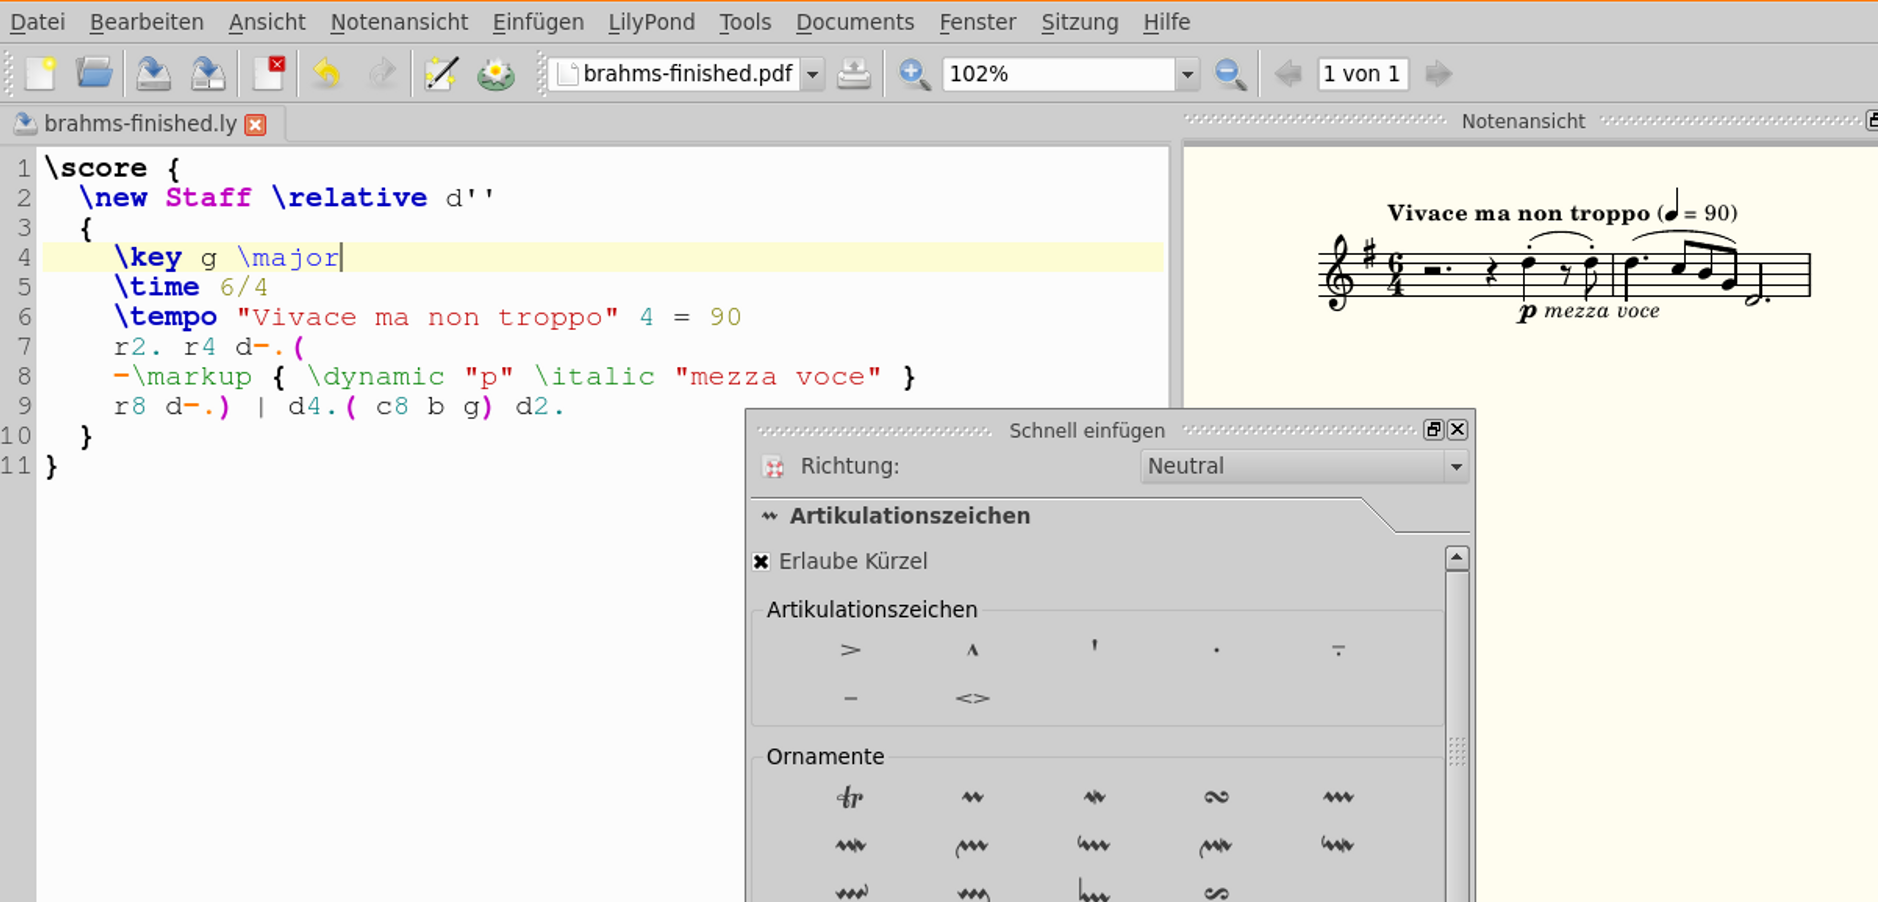
\includegraphics[max width=\textwidth]{examples/frescobaldi-main}
	\caption{Hauptfenster von Frescobaldi, mit Partituranzeige, Quelltext-Editor und Werkzeugleisten}
	\label{fig:pt_fb-main-window}
	\end{figure}
Der Editor vereinfacht die Arbeit durch farbige Darstellung der Struktur (\emph{syntax highlighting}) und bietet Funktionen wie die automatische Vervollständigung von Befehlen oder einfache Navigation im Quelltext.
Besonders wichtig ist jedoch die automatische Verknüpfung zwischen Quelltext und Partitur, die es ermöglicht, in der Partitur ein Element anzuklicken, wodurch die Einfügemarke automatisch an die entsprechende Stelle im Quelltext gebracht wird.
Daher ist es inzwischen nicht mehr problematisch, in komplexen Dateien die Übersicht zu behalten.

Ein Fokus der Entwicklung von Frescobaldi liegt derzeit darin, der Partiturdarstellung größere Funktionalität zu vermitteln.
So wird beispielsweise daran gearbeitet, Tonhöhen direkt in der Partitur  korrigieren oder Bögen und ähnliche Elemente grafisch anpassen zu können.
Die Tendenz geht allgemein dahin, die Arbeit mit Partituren komfortabler zu gestalten und dabei die Vorzüge des textbasierten Ansatzes nicht zu verlieren.

\section{Variablen und eingebundene Dateien}
\label{sec:pt_variables-includes}
In einer LilyPond-Eingabedatei wird die Struktur der Partitur textlich definiert.
Ein grundlegender \cmd{score}-Block sieht etwa folgendermaßen aus:

\begin{quote}
\begin{minipage}{\textwidth}
\begin{verbatim}
\score {
  \new Staff { ... Musik ... }
  ...
}
\end{verbatim}
\end{minipage}
\end{quote}

Anstatt nun -- wie im Screenshot zu sehen -- den musikalischen Inhalt direkt in die Definition des Notensystems einzufügen, wird man diesen in einer \emph{Variablen} notieren und im Notensystem lediglich darauf \emph{verweisen}, sobald die Partitur eine gewisse Komplexität erreicht.
Dies mag auf den ersten Blick wie ein syntaktisches Detail wirken, hat aber ganz erhebliche Auswirkungen auf die Arbeit mit dem Material:
Ging es weiter oben (Abschnitt \ref{sec:pt_separation-content-meaning-appearance} auf S.\,\pageref{sec:pt_separation-content-meaning-appearance}) um die Unterscheidung von \emph{Inhalt} und \emph{Erscheinungsbild}, so handelt es sich hier um die \emph{Definition} und (Wieder-)\emph{Verwendung} des musikalischen Inhalts.
Musik, die in einer Variablen definiert ist, wird in einer Partitur verwendet.
Und sie kann ebenso in einer anderen Partitur verwendet werden.
Durch diese grundsätzliche Herangehensweise kann eine anders kaum mögliche Stabilität beim Herstellen von Einzelstimmen oder Transposition erreicht werden.
Einmal definiertes Material kann beliebig wiederverwendet werden.

\medskip
Eine erhebliche Erweiterung ihres Potenzials erhalten Variablen durch die Möglichkeit, in separate Dateien ausgelagert zu werden, die durch einen \cmd{include}-Befehl in das zentrale Partiturdokument integriert werden.
Nicht nur Musik, auch Formatierungsbefehle oder manuelle Layoutanpassungen können auf diese Weise \emph{wiederverwendet} werden, und es können -- ähnlich den bekannten \emph{Cascading Style Sheets (\textsc{css})} im Webdesign -- komplexe und mächtige Szenarien entwickelt werden.
So können etwa Stildefinitionen hierarchisch auf globaler, Haus-, Projekt- und Dateiebene verwaltet werden -- Änderungen etwa der Projekt-Stilvorlage wirken sich dann automatisch auf alle Partituren des Projekts aus.
Ebenso kann etwa durch den Austausch einer einzigen \cmd{include}-Anweisung zwischen Layouteinstellungen für Partitur, Einzelstimme, Studienpartitur oder Projektor gewechselt werden.
Denkbar und nützlich ist beispielsweise auch ein Entwurfsmodus, bei dem während der Entwicklung der Partitur Herausgeberzusätze farblich hervorgehoben werden und der Zeilen- und Seitenumbruch der Originalvorlage übernommen wird.
Darüber hinaus können hauseigene oder projektbezogene Funktionsbibliotheken erstellt und gepflegt werden.

\section{Kommentare}
\label{sec:pt_lilypond-comments}
Wie bei jedem Texteingabeformat können auch in LilyPond-Dateien \emph{Kommentare} in den Quelltext eingefügt werden, die bei der Übersetzung ignoriert werden.
Diese dienen zunächst der Dokumentation und Erläuterung des Quelltextes, können aber auch zur Kommentierung und Diskussion des Inhalts verwendet werden und beispielsweise offene Fragen festhalten.

Derzeit wird an einer erheblichen Ausweitung dieses Konzepts mit Blick auf kritische Ausgaben gearbeitet.
In Kürze wird es möglich sein, explizite Kommentare in den Quelltext -- \emph{d.\,h. in unmittelbarer Nähe der Definition des Notentexts} -- einzufügen und von einem Hilfsprogramm zu verschiedenartigen Listen aufbereiten zu lassen.
Auf diese Weise können unmittelbar aus dem Partiturdokument heraus Listen mit \textsc{todo}s, editorischen und typografischen Fragen und schließlich auch kritischen Anmerkungen erzeugt werden.
Von den Listeneinträgen führen Links direkt an die entsprechende Stelle im Quelltext.
Geplant ist darüber hinaus, die Kommentare direkt in Frescobaldis Partituransicht bearbeiten zu können -- somit wird es möglich, die gesamte Vorbereitung einer kritischen Ausgabe \emph{innerhalb der konkreten Partitur} durchführen zu können!
Schließlich wird es sogar Möglichkeit sein, die in der Partitur gespeicherten Einträge zum kritischen Bericht direkt in eine schriftliche Fassung exportieren zu lassen.

\section{Programmierbarkeit}
\label{sec:pt_lilypond-programmability}
Weiter oben auf S.\,\pageref{sec:pt_programmability} habe ich über den programmatischen Zugriff auf Textdateien gesprochen.
Dies trifft selbstverständlich auch auf LilyPond-Dateien zu, wobei auf zwei Ebenen programmiert werden kann:
Einerseits verfügt LilyPond mit Scheme%
\footnote{\url{http://de.wikipedia.org/wiki/Scheme}}
über eine mächtige und praktisch unbeschränkte Erweiterungssprache, mit der die Funktionalität des Programms fundamental erweitert werden kann (ein Großteil der eingebauten Funktionalität selbst basiert auf Scheme)%
\footnote{So zeigt etwa Nicolas Sceaux in einer Reihe von Blog-Beiträgen, wie LilyPonds Notation um historische Ornamente erweitert werden kann, die dann als Befehle genauso wie die eingebauten zur Verfügung stehen: \url{http://lilypondblog.org/2013/08/adding-ornamentations-to-note-heads-part-1/}}.
Andererseits können die Eingabedateien selbst mit beliebigen Programmiersprachen bearbeitet oder generiert werden.

Für den normalen Umgang mit LilyPond sind selbstverständlich keine Programmierkenntnisse erforderlich, jedoch öffnet die Programmierbarkeit Perspektiven für größere Projekte.
Und in solchen kann die komplexe Programmierung von wenigen Spezialisten übernommen werden, um der Mehrzahl der normalen Mitarbeiter eine einfachere Arbeitsumgebung zu bieten.
Derzeit arbeite ich zum Beispiel an der Edition eines großen Orchesterwerks%
\footnote{Oskar Fried: \emph{Das trunkne Lied}, siehe \url{http://lilypondblog.org/2013/06/das-trunkne-lied/}}.
Dieses Projekt ist so eingerichtet, dass der einzelne Bearbeiter jeweils nur mit einem kurzen Segment (d.\,h. dem Inhalt einer Stimme im Umfang einer Probenziffer) konfrontiert ist.
Die Partitur und die Einzelstimmen können zu jedem Zeitpunkt erzeugt werden und verwenden in einer von Pausen erfüllten Partitur alle bereits eingegebenen Segmente.
Die Arbeit kann so einerseits beliebig „parallelisiert“ werden und andererseits von Personen erledigt werden, die möglicherweise mit der Bearbeitung einer ganzen Partitur überfordert wären.

\bigskip
\hrule
\bigskip

Durch die in diesem Kapitel beschriebenen Eigenschaften bietet sich LilyPond in hervorragender Weise für die musikwissenschaftliche Editionspraxis an.
Dabei steht die Erörterung der Integrationsmöglichkeiten mit Textsatz durch \LaTeX{} noch aus, und das Potenzial der Versionskontrolle sollte an dieser Stelle noch einmal hervorgehoben werden.

Es gibt allerdings derzeit noch einen Schönheitsfehler, der leider nicht unterschlagen werden kann: den Datenaustausch mit anderen Notensatzprogrammen.
Momentan ist die Verwendung von LilyPond noch eine Einbahnstraße, deren einziger „Ausgang“ die verschiedenen grafischen Partiturformate sind.
So ist es zwar möglich, Partituren aus anderen Programmen in LilyPond-Eingabedateien zu konvertieren, nicht dagegen, eine in LilyPond eingegebene Partitur in Formate zu exportieren, die von anderen Notationsprogrammen gelesen werden können.
Dies ist insofern ein großes Problem, als die Mehrzahl der Verlage auf Dateien der beiden großen grafischen Programme besteht und LilyPond-Dateien nicht akzeptiert.

Auf Grund des bisher Beschriebenen sollte deutlich sein, dass die Vorbereitung von Notenausgaben mit LilyPond auch dann äußerst sinnvoll ist, wenn die endgültige Druckvorbereitung mit \emph{Fin}ale oder \emph{Sibelius} durchgeführt würde.
Daher ist die Ergänzung einer Exportmöglichkeit in das gebräuchliche Austauschformat MusicXML eines der wichtigsten Desiderata der LilyPond-Entwicklung aus musikwissenschaftlicher Perspektive.
Diese scheint dabei kein grundsätzliches technisches Problem, sondern „nur“ eine Frage der Ressourcen zu sein -- für eine grundlegende Implementierung wären wohl lediglich einige Wochen Arbeit eines einzelnen Programmiers erforderlich.
\emph{Ein} größeres Projekt wäre möglicherweise genug, um in dessen Rahmen sowohl den MusicXML-Export als auch die zuvor beschriebene Erweiterung der Quelltextkommentierung zufriedenstellend zu realisieren \dots


\chapter{\LaTeX}
\label{chap:pt_latex}

\LaTeX%
\footnote{\url{http://www.latex-project.org}}
ist für Textdokumente, was LilyPond für Partituren ist:
es bietet Text\emph{satz}, im Gegensatz zu bloßer Text\emph{verarbeitung}.
Wem an guter Typografie gelegen ist, wird \LaTeX{} lieben, wer ihr aber keine Bedeutung beimisst, sollte bedenken, dass „keine Typografie“ nicht möglich ist -- sie wirkt \emph{immer}. 

Mit Textverarbeitungsprogrammen wie Word oder OpenOffice ist es unmöglich, professionell gesetzte Dokumente zu erstellen, insofern ist \LaTeX{} eher in Konkurrenz zu \textsc{dtp}-Programmen wie InDesign oder QuarkXPress zu sehen.
Hinsichtlich der Qualität zumindest bei Textdokumenten muss man bei der freien Software keinerlei Abstriche machen, im Gegenteil bietet sie gerade hinsichtlich der Mikrotypografie ganz hervorragende Möglichkeiten.
Einzig bei grafisch komplexen Aufgaben wie Plakaten oder vielleicht Buchcovern könnte die Wahl auf ein grafisch orientiertes Programm fallen.
Da \LaTeX{} ursprünglich für den Buchsatz entwickelt und seit Jahrzehnten verbessert wurde, bietet es selbstverständlich professionelle Möglichkeiten für Literaturverwaltung, Zitate, Indizes etc.
Darüber hinaus bietet \LaTeX{} alle Vorzüge, die ich für textbasierte Softwaresysteme im Allgemeinen beschrieben habe.

Die Schnittstelle zu \LaTeX{} ist ähnlich wie bei LilyPond:
Eingabedateien mit einer ähnlichen Syntax werden in \textsc{pdf}-Dateien \emph{übersetzt}.
Auf Grund des Alters des Systems existieren zahllose Bearbeitungsprogramme unterschiedlichen Zuschnitts und Komforts.
Die Eingabesprache bietet \emph{Befehle} und \emph{Umgebungen}, die entfernt mit Text- und Absatzvorlagen von Textverarbeitungsprogrammen vergleichbar, jedoch ungleich mächtiger sind:
Sie reichen von einfacher semantischer Auszeichnung über (etwa) Abbildungen, die nach traditionellen Satzregeln im Text positioniert werden bis hin zu komplexen Befehlen mit mehreren Argumenten.

Eine noch so oberflächliche Einführung in \LaTeX{} würde den Rahmen dieses Textes sprengen, daher beschränke ich mich auf einige Hinweise zu spezifisch musikalischen Aspekten.


\section{Musikbeispiele}
\label{sec:pt_music-examples}

\LaTeX{} ist in der Lage, Abbildungen satztechnisch hochwertig einzufügen und hat auch keine Schwierigkeiten mit einer Vielzahl von Bildern in langen Dokumenten.
Zur Verwaltung von Notenbeispielen gibt es jedoch einige speziellere Werkzeuge, insbesondere \package{lilypond-book} and \package{musicexamples}.

\package{lilypond-book} ist ein Hilfsprogramm, das gemeinsam mit LilyPond ausgeliefert wird und ermöglicht, LilyPond-Code direkt in \LaTeX-Dokumente einzufügen.
Beim Durchlauf werden die Notenbeispiele bei Bedarf neu erzeugt und der Quellcode durch entsprechende Bilddateien ersetzt.
Der potenzielle Nachteil an diesem Ansatz ist, dass die zu bearbeitende Datei nicht direkt von \LaTeX{} übersetzt werden kann, sondern zunächst von \package{lilypond-book} vorverarbeitet werden muss.
Für Dokumente mit vielen kurzen Notenbeispielen kann es jedoch die effektivste Möglichkeit sein, die Noten \emph{in situ} zu verwalten.

Demgegenüber versteht sich \package{musicexamples}%
\footnote{\url{http://www.openlilylib.org/musicexamples}} 
als ein Werkzeug, das sich mehr der Einbettung und konsistenten Verwaltung von Notenbeispielen widmet.
Besonderes Augenmerk wurde auf den Umgang mit ganz- und mehrseitigen Notenbeispielen gelegt, für eine weitergehende Integration speziell von LilyPond-Partituren existieren konkrete Pläne.
Insbesondere ist mittelfristig vorgesehen, mit Hilfe der in \hologo{LuaLaTeX} verwendeten Programmiersprache \emph{Lua} ebenfalls die Einbettung von LilyPond-Quellcode zu ermöglichen -- allerdings dann ohne den Umweg über ein zwischengeschaltetes Hilfsdokument.

\section{Notationselemente}
\label{sec:pt_notational-elements}
Mit Hilfe des Pakets \lilyglyphs%
\footnote{\url{http://www.openlilylib.org/lilyglyphs}}
ist es möglich, \emph{jegliche} mit LilyPond realisierbare Notationselemente auf Zeichenebene in \LaTeX-Dokumente einzubetten.
Dies können etwa dynamische Zeichen wie \lilyDynamics{mf}, Vorzeichen wie \flatflat{} oder auch grafische Zeichen wie \crescHairpin{} oder Taktbezeichnungen (\lilyTimeSignature{4+3}{8} oder \lilyTimeCHalf) sein.
Mit etwas größerem Aufwand kann man auch individuelle Notationen erstellen und einbinden.
Das Schöne daran ist, dass man mit dem Paket auf den \emph{gesamten} Notationsvorrat von LilyPond in dessen hervorragender Qualität zugreifen kann, die verwendeten Zeichen problemlos mit dem Text fließen und sich leicht in Größe und Positionierung anpassen lassen.

\bigskip
Ideen für weitere Erweiterungspakete, die bei konkretem Bedarf jederzeit in Angriff genommen werden können, umfassen beispielsweise funktionsharmonische Analysesymbole oder Generalbassbezifferungen.

\chapter{Anwendungsbeispiele}
\label{chap:pt_applications}

Die Anwendungsbeispiele erörtern abschließend die beschriebenen Programme und Konzepte in ihrem Zusammenspiel und ihrer Potenziale speziell für musikwissenschaftliches Arbeiten.
Andere Anwendungsgebiete wie etwa im didaktischen Bereich entsprechen dagegen nicht dem Hauptzweck dieses Aufsatzes.

\section{Vorbereiten einer Notenedition}
\label{sec:pt_preparing-edition}
Die Erarbeitung einer Notenedition werde ich als ausführlichsten Anwendungsfall beschreiben, da dieser mir am nächsten liegt.
Die meisten angesprochenen Aspekte sind jedoch für die anschließend genannten, nur oberflächlicher erläuterten Anwendungen ebenso relevant.

\medskip
 
Der Hauptgedanke, der allen weiteren zugrunde liegt, ist das \emph{gemeinschaftliche} Bearbeiten einer geteilten \emph{Datenbasis} von der ersten Skizze über Noteneingabe und kritische Revision bis zu den Druckvorlagen.
Da das Versionskontrollsystem alle Bearbeitungsschritte lückenlos und nachvollziehbar dokumentiert, können die im Rahmen des Projekts anfallenden Aufgaben flexibler verteilt werden als in traditionellen Arbeitsprozessen.
Während es nach wie vor für jedes Fachgebiet Spezialisten geben sollte, können diese ihre Kompetenz auch anderen Teilaufgaben zur Verfügung stellen.
Das verteilte Arbeiten erhöht die Effizienz, da häufig Wartezeiten durch „Dateisperren“ bzw. das Warten auf die Fertigstellung einer Teilaufgabe durch einen anderen Mitarbeiter entfallen.
Gleichzeitig kann aber auch der kreative Austausch angeregt werden, wenn beispielsweise der Notensetzer einen Blick auf editorische Fragen wirft, während sich der Herausgeber an notentypografischen Problemstellungen versuchen kann.
Darüber hinaus stellt Versionskontrolle auch explizit Werkzeuge zur Verfügung, um verschiedene Modelle von \emph{peer review} zu befördern.

Als sehr fruchtbar hat sich die Entwicklung eines „Entwurfsmodus“ bei der Partiturausarbeitung erwiesen.
Gemeinsam mit der Möglichkeit, durch Quelltextkommentare einen Kommunikationskanal zwischen den Projektbeteiligten zu eröffnen, verbessert der Entwurfsmodus den Überblick über das Projekt erheblich.
Die Entwicklung der erweiterten Anmerkungen im Rahmen des \package{lilypond-doc}-Projekts werden diesen Vorteil noch einmal deutlich ausweiten.

Da sich die gesamte Layoutgestaltung in \cmd{include}-Dateien abspielt, ist es annähernd egal, in welcher Projektphase das äußere Erscheinungsbild entwickelt wird, es gibt in dieser Hinsicht kaum Einschränkungen.
Es ist beispielsweise möglich, das Layout der Edition \emph{parallel} zur inhaltlichen Ausarbeitung zu entwickeln, oder aber, für die Arbeitsphasen der Noteneingabe, kritischen Revision und Druckvorbereitung ganz unterschiedlich angepasste Partiturlayouts zu verwenden.

Die Vorbereitung des endgültigen Notenbandes als LaTeX-Dokument(e) kann selbstverständlich ebenfalls in derselben Datenbasis durchgeführt werden.
Als sehr hilfreich erweisen sich hierbei die guten Integrationsmöglichkeiten von Text- und Partiturteilen, seien es ganzseitige Partituren oder kleine Notenbeispiele.

\section{Bücher und Periodika}
\label{sec:pt_books-periodicals}
Was für Noteneditionen gilt, ist für schriftliche Publikation ebenso relevant.
Tatsächlich ist in vielen natur- und computerwissenschaftlichen Disziplinen \LaTeX{} der de-facto-Standard der Einreichung von Texten für Zeitschriften oder Sammelbände.
Beim Abfassen und veröffentlichen schriftlicher Arbeiten erweist sich die Versionskontrolle als perfektes Instrument der Qualitätssicherung und der Kommunikation zwischen Autor und Lektor oder zwischen mehreren Autoren.
Änderungsvorschläge sind -- als \emph{commit} aufbereitet -- unmittelbar verständlich und können übernommen, verworfen oder überarbeitet werden.
Ein gemeinsamer Datenbestand motiviert den Autor, auch nach der ursprünglichen Abgabe aktiv an der Perfektionierung des Texts mitzuwirken.
Und überhaupt erhöht ein ständiger Austausch nicht nur die Perfektion im Detail, sondern auch das kreative Potenzial des/der Autoren.

\section{Längerfristige Projekte}
\label{sec:pt_longrunning-projects}
Auf Grund der langfristigen Stabilität eines textbasierten Datenbestands sowie der guten Integrationsmöglichkeiten der verschiedenen Komponenten bieten sich textbasierte Ansätze auch für langfristige akademische Unternehmungen wie Forschungsprojekte oder Gesamtausgaben an.
Gerade diese können von den Implikationen gemeinschaftlichen (Be-)Arbeitens profitieren, und auch personelle Änderungen können leichter aufgefangen werden, wenn nicht jeder Mitarbeiter sein privates Ordnungssystem hat.
So ist es -- zumindest von der technischen und logistischen Seite her betrachtet -- ohne Weiteres möglich, die Arbeit eines Herausgebers zu übernehmen und nahtlos fortzusetzen.


\section{„Single Source Publishing“}
\label{sec:pt_single-source-publishing}
Bedenkenswert (wenn auch an dieser Stelle nicht näher ausgeführt) ist in diesem Zusammenhang auch, dass neben Text- und Notensatz natürlich auch andere Techniken zum Zuge kommen können, so etwa Datenspeicherung in Datenbanken sowie deren Aufbereitung in Netzwerk- und Internettechnologien.
Das zukunftsträchtige Schlagwort des \emph{Single Source} oder \emph{Cross Media Publishing} ist hierbei eine fast zwangsläufig auftretende Assoziation.
Textbasierte Arbeitsprozesse bieten eine hervorragende Materialgrundlage für die Verarbeitung allgemeiner Inhalte für verschiedene Medien.
Das mag von der Aufbereitung eines kritischen Berichts für eine Web-Abfrage bis zu interaktiven Partituren reichen.

\section{„Crowd Editing“}
\label{sec:pt_crowd-editing}
Ein bislang weitgehend unbekanntes Phänomen lässt sich mit dem künstlich geprägten \emph{Crowd Editing} beschreiben.
Wie bereits weiter oben angesprochen wurde, lassen sich mit Hilfe von Versionskontrolle viele Aufgaben auf eine beliebige Anzahl von Teilnehmern verteilen.
So wird man zwar eine kritische Revision nicht beliebig „clustern“ können, da es selbstverständlich erforderlich ist, den geistigen Zusammenhang zu bewahren.
Tätigkeiten wie Noteneingabe oder Fehlerkorrektur können dagegen ohne weiteres in kleine Portionen aufgeteilt werden.

Ein erfolgreiches Beispiel derartigen Arbeitens ist eine holländische Gesangbuch-Ausgabe%
\footnote{\url{http://www.liedboek.nl}},
die kürzlich mit einer Vielzahl unabhängiger Beitragender einen 1.600 Seiten umfassenden Notenband in nur einem Jahr fertigstellte.

\end{document}